%%%% Proceedings format for most of ACM conferences (with the exceptions listed below) and all ICPS volumes.
\documentclass[sigconf]{acmart}
%%%% As of March 2017, [siggraph] is no longer used. Please use sigconf (above) for SIGGRAPH conferences.

%%%% Proceedings format for SIGPLAN conferences 
% \documentclass[sigplan, anonymous, review]{acmart}

%%%% Proceedings format for SIGCHI conferences
% \documentclass[sigchi, review]{acmart}

%%%% To use the SIGCHI extended abstract template, please visit
% https://www.overleaf.com/read/zzzfqvkmrfzn

\usepackage{booktabs} % For formal tables
\usepackage{graphicx}


% Copyright
%\setcopyright{none}
%\setcopyright{acmcopyright}
%\setcopyright{acmlicensed}
\setcopyright{rightsretained}
%\setcopyright{usgov}
%\setcopyright{usgovmixed}
%\setcopyright{cagov}
%\setcopyright{cagovmixed}


% DOI
\acmDOI{10.475/123_4}

% ISBN
\acmISBN{123-4567-24-567/08/06}

%Conference
\acmConference[ACMMM2017]{ACM Multimedia}{October 2017}{Mountain View, CA USA} 
\acmYear{2017}
\copyrightyear{2017}

\acmPrice{15.00}


\begin{document}
\title{Visualising Travel Route via Structured Recommendation}

\author{Dawei Chen}
\orcid{1234-5678-9012}
\affiliation{%
  \institution{Data61 \& The Australian National University}
  \streetaddress{P.O. Box 1212}
  \city{Dublin} 
  \state{Ohio} 
  \postcode{43017-6221}
}
\email{trovato@corporation.com}

\author{G.K.M. Tobin}
\authornote{The secretary disavows any knowledge of this author's actions.}
\affiliation{%
  \institution{Institute for Clarity in Documentation}
  \streetaddress{P.O. Box 1212}
  \city{Dublin} 
  \state{Ohio} 
  \postcode{43017-6221}
}
\email{webmaster@marysville-ohio.com}

\author{Lars Th{\o}rv{\"a}ld}
\authornote{This author is the
  one who did all the really hard work.}
\affiliation{%
  \institution{The Th{\o}rv{\"a}ld Group}
  \streetaddress{1 Th{\o}rv{\"a}ld Circle}
  \city{Hekla} 
  \country{Iceland}}
\email{larst@affiliation.org}

% The default list of authors is too long for headers}
\renewcommand{\shortauthors}{D. Chen et al.}


\begin{abstract}
In this demo, we propose a novel trajectory visualisation tool. 
\end{abstract}

%
% The code below should be generated by the tool at
% http://dl.acm.org/ccs.cfm
% Please copy and paste the code instead of the example below. 
%
\begin{CCSXML}
<ccs2012>
 <concept>
  <concept_id>10010520.10010553.10010562</concept_id>
  <concept_desc>Computer systems organization~Embedded systems</concept_desc>
  <concept_significance>500</concept_significance>
 </concept>
 <concept>
  <concept_id>10010520.10010575.10010755</concept_id>
  <concept_desc>Computer systems organization~Redundancy</concept_desc>
  <concept_significance>300</concept_significance>
 </concept>
 <concept>
  <concept_id>10010520.10010553.10010554</concept_id>
  <concept_desc>Computer systems organization~Robotics</concept_desc>
  <concept_significance>100</concept_significance>
 </concept>
 <concept>
  <concept_id>10003033.10003083.10003095</concept_id>
  <concept_desc>Networks~Network reliability</concept_desc>
  <concept_significance>100</concept_significance>
 </concept>
</ccs2012>  
\end{CCSXML}

\ccsdesc[500]{Computer systems organization~Embedded systems}
\ccsdesc[300]{Computer systems organization~Redundancy}
\ccsdesc{Computer systems organization~Robotics}
\ccsdesc[100]{Networks~Network reliability}

% We no longer use \terms command
%\terms{Theory}

\keywords{ACM proceedings, \LaTeX, text tagging}

% Used in some conference proceedings e.g. sigplan and sigchi
 \begin{teaserfigure}
 \centering
   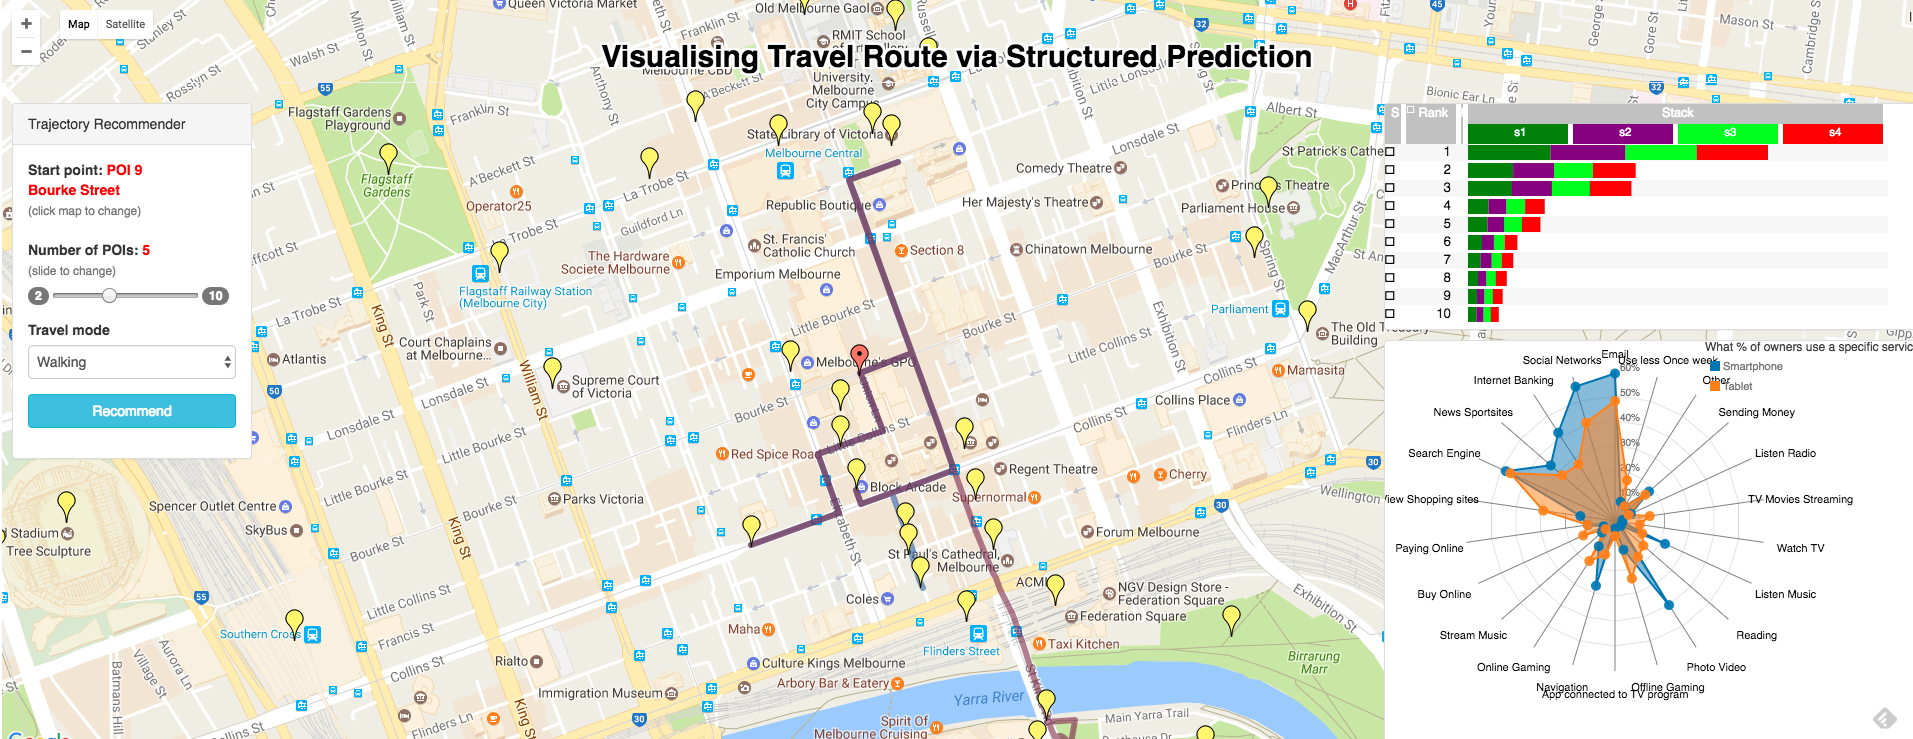
\includegraphics[width=0.8\textwidth]{figure/sample_map.png}
   \caption{Travel route recommendation system. Given a starting POI and a number of POI to be visited, the algorithm suggests a set of routes from a history of previous travellers.}
   \label{fig:overview}
 \end{teaserfigure}

\maketitle


\section{Introduction}
%background
Sequence ranking has emerged as an important tool for solving diverse problems such as travel route and music playlist recommendations. Unlike the classical ranking algorithm where each item considers independently, the sequence ranking algorithm requires modelling a structure between items and suggests a set of items as a whole. For example, let us consider recommending a trajectory of points of interest (POI) in a city to a visitor. If the classical ranking algorithm learns a user's preference for each individual location while ignores the distances between them, the algorithm may create a long trajectory, which should be shorter in optimal routeing. Several sequence ranking algorithms are proposed to solve the problem and achieve relative success to compare with the classical algorithms. An important challenge remaining is how to visualise the recommended sequences so that a user can understand why the sequences are suggested.

%approach
In this paper, we tackle the problem of sequence visualisation, especially, in the context of a travel route recommendation. We first formulate the sequence ranking algorithm as a structured recommendation problem, and then we develop a novel visualisation engine that efficiently distinguishes differences between suggested routes as well as a variation of POIs within a suggested route. 

\section{Structured Recommendation}
%what is special about sr?
We solve the sequence ranking algorithm


\section{Visualisation}
%what are the features we want to emphasis?
%make a bullet list of something like that
Break total score into individual feature score, represent using stacked bar graph.

Comparison between two POIs in a single trajectory.
Further comparison of POIs within a single trajectory, we use radar chart to show the score of each feature.


\begin{figure}[t!]
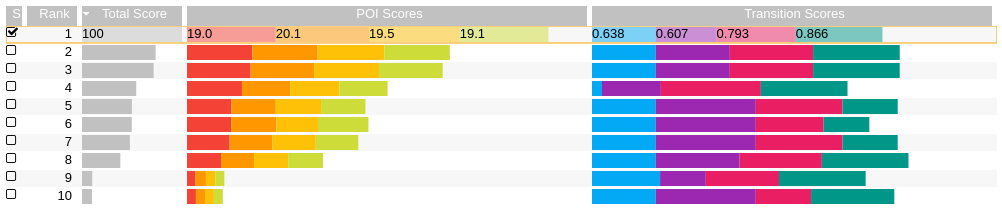
\includegraphics[width=0.9\linewidth]{figure/sample_stack.png}
\caption{Visualisation of feature score for each trajectory.}
\end{figure}

\begin{figure}[t!]
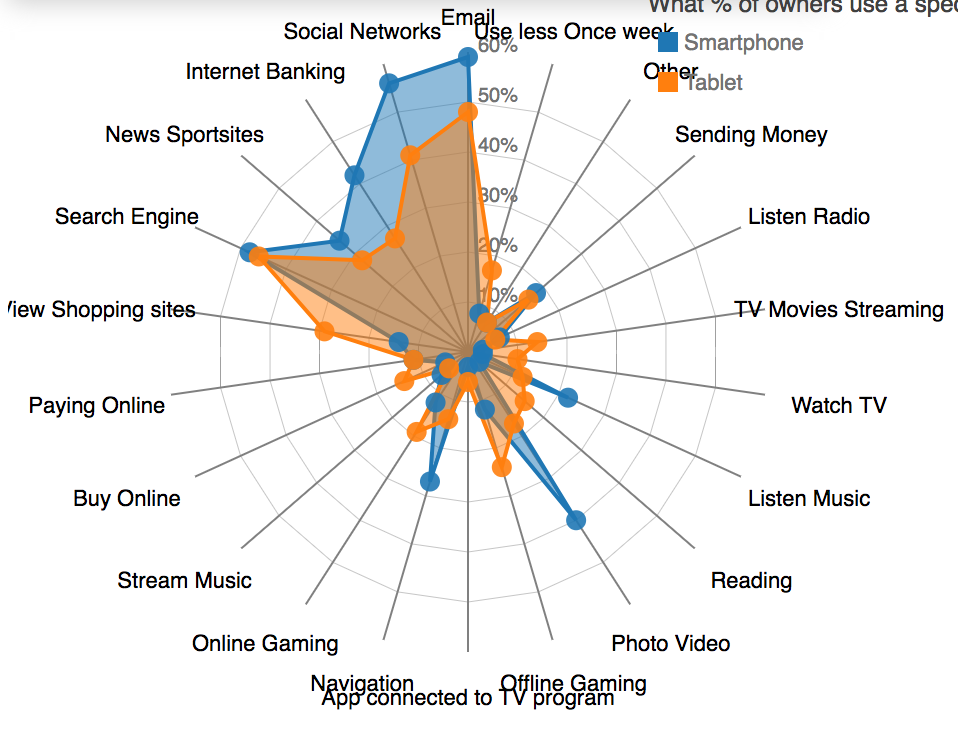
\includegraphics[width=0.9\linewidth]{figure/sample_radar.png}
\caption{Visualisation of feature score for each POI within a single route.}
\end{figure}


\section{Conclusion}
%summary


\bibliographystyle{ACM-Reference-Format}
\bibliography{sigproc} 

\end{document}
